\documentclass{tufte-handout}
\title{Chapter 3: Processes}
\author{Andr\'es Ponce}
\usepackage{graphicx}
\graphicspath{ {./img/} }

\begin{document}
\maketitle

\begin{abstract}
A \textbf{process} is a program that is currently running.
One of the main functions of an operating system is to run user programs,
so the way an OS manages process execution, scheduling and memory management
can become quite important.
\end{abstract}

The status of the current executing program can be known with the value of the 
\textbf{program counter}
\footnote{The PC stores the address of the currently executing instruction.}
and the values currently in the registers.

Usually, a program executable file has four distinct sections. The \textbf{text section}
contains the executable code, while the \textbf{data section} contains the global 
variable declarations. the \textbf{heap} is where the dynammic memory is allocated, and 
the \textbf{stack} is where temporary variables are allocated. These variables are the ones
used for function executions and are then deleted.

The data and text sections of a program are fixed, since they do not change during execution.
However, the stack and heap shrink as needed, and they grow \textbf{toward} each other but
never \textbf{overlap} each other. \footnote{Then how do we account for really big programs?}

The program state can fall into certain categories:
\begin{itemize}
	\item \textbf{New}: Process is being created.
	\item \textbf{Running}: There are instructions being executed.
	\item \textbf{Waiting}: Process is waiting for some event.
	\item \textbf{Ready}: Process is ready to be assigned to CPU.
	\item \textbf{Terminated}: Process finished execution.
\end{itemize}

\subsection{Process Control Block}
The proces is represented in the OS by using a block of memory containing program info called
the \textbf{Process Control Block}. It stores a couple things:
\begin{itemize}
	\item \textbf{Process State}: One of previously mentioned process state.
	\item \textbf{Program Counter}: Address of the next instruction to be executed.
	\item \textbf{CPU registers}: There are different types of registers that store different
				information. This has to be saved on interrupt to be able to resume when the 
				interrupt is resolved.
	\item \textbf{CPU scheduling}: Scheduling parameters.
	\item \textbf{Mem. Mgmt. Information}: The value of the base and limit registers, page tables, 
				segment tables, depending on memory scheme in computer.
	\item \textbf{Accounting Information}: Amount of CPU and real time used, time limits, 
				process/job numbers, etc...
	\item \textbf{I/O Status Information}: List of open files, I/O devices allowed to use, etc...
\end{itemize}

The set of PCB's is stored as a linked-list, with the info stored in \texttt{include/linux/sched.h}.
When we want to schedule a process, we have to change the state. Then we execute until we are
finished or waiting for a process, and move to the next program in the \textbf{wait queue}.

In terms of scheduling, each process gets a CPU core when it needs to and gets removed when 
not in need of execution, such as waiting for I/O. For CPU bound instructions though, they also 
don't get to execute constantly throughout its lifetime, the CPU scheduler might forcible remove
it after a specified time limit. 

When changing the CPU core from execution of one process to another, most systems will save the 
current state of the executing program and load the state of the program to execute. This 
switching of process is known in the biz as \textbf{context switching}, since the state of the 
registers and execution point of a program when saved and loaded can be called the context.
\begin{marginfigure}
		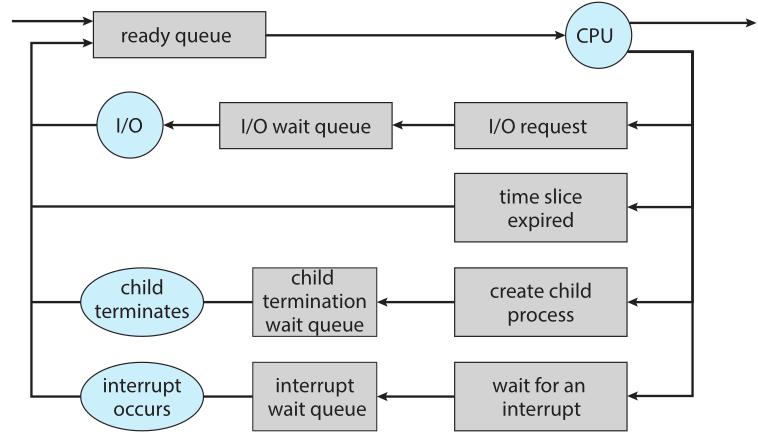
\includegraphics[scale=0.3]{queueing}
		\caption{For an active process, the process may be not executing while it's
		waiting for I/O, or while it's waiting for interrupt. During execution,
		this program might be descheduled to allow other ready programs to execute.
		It's taken off the ready queue.}
\end{marginfigure}
\section{Operations on Processes}
When executing, each process on Windows and UNIX gets a unique \textbf{process identifier}, 
\footnote{a.k.a. pid}
which uniquely identifies the process in the kernel. Since each process can spawn other 
children processes, the execution diagram can become an execution \textbf{tree}. In Linux, 
the \texttt{systemd} process always has a pid of 1. This process is the only user program
run at boot time, and every process starts under the systemd node in the execution tree. 
The \texttt{logind} process manages the clients that are logged in to the system.

What happens when we create/run a program? First, the OS is responsible for allocating
the resources the process needs to operate. Remember that a process can have another
process execute inside of it called a \textbf{child process}. Since the parent has some
execution and read/write permissions, as well as some data, the child process inherits 
some of them. However, the child's processes are to be a \textbf{subset} of the parents',
and this is done to discourage the creation of unnecessary processes.
Child processes will overlay their memory footprint with that of the parents, so that 
they occupy some of the same address space as the parents. Also, during execution of 
the child process, the parent's \texttt{pid} is replaced with that of the child. 
The child technically has a \texttt{pid} of 0, although its true one is taken on by 
the parent.

How do processes terminate? When they reach the final statement to be executed, they
call on the \texttt{exit()} system call. Parents can also terminate their own
children, but cannot terminate other programs. Why would a parent terminate its 
child process? Maybe the child's available resources have been exceeded, or the child
process is simply no longer needed. If the parent is executing, we also need 
the child process to execute as well, since the OS usually does not permit parent
processes to terminate while their children are still executing.

\subsection{Android Process Hierarchy}
In the Android operating system, instead of terminating arbitrary processes, there
is a hierarchy of importance. The motivation for this is that mobile systems need to 
aggressively control memory and thus need to constantly be reclaiming system resources. 
The categories of importance in Android includes 
\begin{itemize}
	\item \textbf{Foreground process}: This process is the one currently occupying the user's 
			screen.
	\item \textbf{Visible process}: A process that is not visible on the screen but that 
			performs a function whose result is displayed on the foreground process.
			\footnote{Are these the processes spawned by the foreground process?}
	\item \textbf{Background process}: Process that performs an activity not apparent 
			to the user.
	\item \textbf{Empty Process}: Process not associated with any application.
\end{itemize}

\section{Interprocess Communication in Shared Memory}
Previously, we had mentioned two models for interprocess communication: shared memory and
message passing. In the shared memory model, a region in memory is designated as memory that 
both processes can use to store info they want passed. In the message passing model, we can 
directly send a message between the two programs.
\footnote{Is this where sockets or system links come in?}
Shared memory is usually faster than message passing becuase message passing can involve many
system calls and be overall slower. However, the process to use shared memory is up to the 
processes and not the OS, so they have to both make sure they handle it correctly and are not 
writing to the same region simultaneously.

In shared memory, there is a \textbf{producer} and \textbf{consumer}. The producer makes some
info that the consumer will read. For example, a compiler will produce some code that might
be read by the assembler and the assembler in turn produces machine code to be executed. Thus
for the producer-consumer model we also need a way to model it in the memory buffer. The two
processes will use a memory buffer of certain size to communicate. This might be a 
\textbf{bounded} or \textbf{unbounded} buffer, in which there is no strict size limit.
In case of a bounded buffer, the consumer might have to wait for new stuff from the producer and
likewise the producer will have to wait if the buffer is full before putting in new 
information.

\section{Interprocess Communication in Message-Passing Systems}
How do we pass along information which may be used by two different systems, or two different
computers. We need some \textbf{communication link} in order to send the messages. 
We could have a scheme in which a message-passing system calls a function like 
\texttt{send(P, message)} to sendmessage \texttt{message} 

Another scheme involves using \textbf{ports} or \textbf{mailboxes}. Similar to mail protocols, 
the mailbox and ports involve placing a message there and the message being read at some point
by the other program. So in this scheme we send and receive messages from the mailbox. The 
owner process will start the mailbox and then the mailbox's access info might be passed to the
requesting program.

Processes might either be \textbf{synchronous} or \textbf{asynchronous}. These two terms 
refer to whether the message has to be read by the othe process before being able to write 
to the process again. 

The messgaes, when they arrive at a port, will be placed in a queue. In UNIX we use the 
\texttt{mach\_msg()} to indicate if the current port is a receiver or sender process.

In Windows, if we wish for two processes to communicate, we have to communicate with a 
\textbf{subsystem server}, which assigns a channel for the process to use.
\end{document}
